\documentclass[a4paper, 12 pt]{article}

\usepackage{amsfonts}
\usepackage{amsmath}
\usepackage{amsthm}
\usepackage{appendix}
\usepackage{bm}
\usepackage{booktabs}
\usepackage[usenames, dvipsnames]{color}
\usepackage{graphicx}
\usepackage{epstopdf}
\epstopdfsetup{update}
\usepackage{helvet}
\usepackage{hyperref}
\usepackage{indentfirst}
\usepackage{lscape}
\usepackage{morefloats}
\usepackage{natbib} \bibliographystyle{ecta}
%\bibliographystyle{abbrvnat}\bibpunct{(}{)}{;}{a}{,}{,}
\usepackage{setspace}
\usepackage{subcaption}
\usepackage[capposition=top]{floatrow}
\usepackage{subfloat}
\usepackage[latin1]{inputenc}
\usepackage{tikz}
%\usepackage[pdf]{pstricks}

\usetikzlibrary{trees}
\usetikzlibrary{decorations.markings}


\theoremstyle{plain}
\newtheorem{thm}{Theorem}
\newtheorem{cor}{Corollary}
\newtheorem{lem}[thm]{Lemma}
\newtheorem{proposition}{Proposition}
\newtheorem{assumption}{Assumption}
\newtheorem{definition}{Definition}

%MARGINS
 \topmargin   =  0.0in
 \headheight  =  -0.3in
 \headsep     =  0.7in
 \oddsidemargin= 0.0in
 \evensidemargin=0.0in
 \textheight  =  9.0in
 \textwidth   =  6.45in
%\setlength{\parindent}{4em}
%\setlength{\parskip}{1em}

\newcommand{\fmt}{.eps}
%\newcommand{\fmt}{.png}
\hypersetup{
    colorlinks=true,
    linkcolor=BlueViolet,
    citecolor=BlueViolet,
    filecolor=BlueViolet,
    urlcolor=BlueViolet
}




\setcounter{page}{0}
\begin{document}



\title{\Large{\textsc{Choosing Season of Birth:}}\\ \Large{\textsc{The Role of Biological and Economic Constraints}}\thanks{\scriptsize{We thank seminar participants at University of Surrey and participants in the ``Family Economics'' Workshop (Barcelona Graduate School of Economics) June 2015 for helpful comments and suggestions. The usual disclaimers apply. Any errors contained in the paper are our own.}}}
\author{\small{Damian Clarke} \\ \small{University of Oxford} \and \small{Sonia Oreffice} \\ \small{University of Surrey \& IZA}  \and \small{Climent Quintana-Domeque} \\ \small{University of Oxford \& IZA}}

\date{\small{September 22, 2015} \\ \vspace{2mm} \small{\textbf{Preliminary Draft}}}

%\author{Damian Clarke  \and Sonia Oreffice  \and Climent Quintana-Domeque  }
%\author{Damian Clarke \\ University of Oxford \and Sonia Oreffice \\ University of Surrey and IZA \and Climent Quintana-Domeque \\University of Oxford and IZA}


\maketitle
\thispagestyle{empty}

\begin{abstract}
We provide novel estimates of women's decision of when to have their first birth in terms of fertility timing (young vs. old) and season of birth (which quarter), for non-Hispanic white women aged 25-45 in the US in 2005-2013. The prevalence of good season (quarters 2 and 3) is very significantly related to mother's age, as well as to her education and marital status, while those who do not undergo assisted reproductive technology procedures to achieve their first birth exhibit a much higher prevalence of good season births. The frequency of good season is also higher and more strongly related to mother's age in states where cold weather is more severe, reinforcing the interpretation that season of birth is a choice outcome. Finally, we perform a structural investigation to quantify the value of good season of birth in terms of birth weight and wages.
\end{abstract}
\emph{JEL Classification Codes}: I10, J01, J13.\\
\emph{Keywords}: quarter of birth, fertility timing, birth outcomes, wages.


\newpage
%\begin{spacing}{1.4}
\begin{doublespace}

%-------------------------------------------------------------------------------
\section{Introduction}
\paragraph{Motivation.} While the relevance of season of birth has been acknowledged at least since \citet{Huntington38} wrote his book ``Season of Birth: Its Relation to Human Abilities'', it was not until the seminal article by \citet{AK1991} --quarter of birth is shown to be related to education and earnings in the US-- that season of birth became popular in economic research. Recent work has unveiled a variety of channels, beyond school cutoff laws, through which season of birth may affect adult outcomes, for example, its potential effects on birth outcomes. Indeed, a clear and consistent pattern of ``good'' and ``bad'' seasons has emerged. In the US, winter months are associated with lower birth weight, education and earnings, while Spring and Summer are found to be ``good'' seasons (e.g., \citealp{BucklesHungerman2013}; \citealp{CS2013}). However, no study so far has considered season of birth as a choice outcome. The purpose of this paper is precisely to fill this gap, by considering season of birth as a decision variable and quantifying the trade-offs that mothers face (if any) when choosing season of birth. To further motivate our approach, we present several novel stylized facts in Figures 1-5 suggesting that season of birth is indeed a matter of choice.

\paragraph{Stylized facts.}  Figure 1 shows the gap between the fraction of first births to ``younger'' (25-39) and ``older'' (40-45) women by month: The gap is positive in the months representing the ``good'' season (April to September) and negative in the ``bad'' season (October to March). This finding is consistent with ``younger'' mothers being less biologically constrained than ``older'' mothers when making their fertility decision, \emph{ceteris paribus}. Figure 2 reveals that, for ``younger'' women, good season is more prevalent in the North of the US than in the South. However, this pattern does not hold for ``older'' women, as we can see in Figure 3. Specifically, among ``younger'' women, a much higher proportion of good season births are observed in the northern states where the winter temperature is more severe. Interestingly, there is a North-South gradient, southern states with milder Winter exhibit lower proportion of births in good seasons. Strikingly, no such geographical pattern is observed of first births to ``older'' mothers, with the proportion of good season births appearing to be unrelated to geographic location of the state.

We further investigate whether the geographical differences in the prevalence of good season are due to weather conditions in Figure 4. If women choose season of birth at all, they may be more willing to give birth in the Spring or Summer, at least in states with more severe cold weather in Winter. We plot the percentage of ``younger'' women giving birth in the good season against the coldest monthly average by state: The pattern is spectacular. There is a strong linear negative association between these two variables (correlation coefficient = $-0.729$). Interestingly, we do not find such a relationship for older women (correlation coefficient = $-0.115$). Finally, in Figure 5, we present additional evidence that the seasonality of births is strongly related to weather: The US (Northern hemisphere) seasonality patterns of birth are completely reversed in Chile (Southern hemisphere).

Given the prominence of fertility planning in balancing people's work and family life as well as the above stylized facts, it is hard to believe that season of birth may simply be a matter of chance. In addition, far from assuming that the average woman is aware that birth weight and the child's future earnings are affected by birth timing, it is sufficient to consider that the average woman has a sense that, on the one hand, winter months may be tougher birth months because of cold weather and higher disease prevalence,\footnote{According to the \citet{CDC2014}, from 1982-83 through 2013-14, the ``peak month of flu activity'' (the month with the highest percentage of respiratory specimens testing positive for influenza virus infection), has been February (14 seasons), followed by December (6 seasons) and January and March (5 seasons each): \href{http://www.cdc.gov/flu/about/season/flu-season.htm}{http://www.cdc.gov/flu/about/season/flu-season.htm}}
and on the other, work commitments make it much easier to take time off with a Spring-Summer birth.\footnote{The report on fertility, family Planning, and women's health (\citealp{CDC1997}) notes that some women do not take maternity leave due to the timing birth relative to their job schedules, and gives the example of school teachers who deliver during summer break.}

\paragraph{This paper.} We first present novel correlates of season of birth, investigating women's decision of when to have their first birth in terms of fertility timing (young versus old) and season of birth (which quarter), for non-Hispanic white women aged 25-45. Using US Vital Statistics data from 2005 to 2013 on all first singleton births, we show that the prevalence of good season (quarters 2 and 3) is very significantly related to mother's age, as well as to her education and marital status. In addition, we find that women who do not undergo assisted reproductive technology (ART) are 3 percentage points more likely to give birth in the good season. This finding, which is robust to controlling for gestation length fixed effects, is consistent with season of birth being a choice outcome, if undergoing ART is associated to no longer being under control of birth timing. Moreover, if women undergoing ART cannot choose season of birth, we should expect to find no seasonality gap, and we present supportive evidence for this prediction. We then examine how birth outcomes, such as birth weight, prematurity ($<37$ weeks of gestation) and APGAR scores, are related to season of birth controlling for mother's characteristics. We find that being born in the good season is positively associated to better birth outcomes.

In the second part of our investigation, we construct a structural model to examine women's decisions of \emph{when in their life cycle} (young vs. old) and \emph{in which season} (good vs. bad) to have the first child. On average, younger mothers deliver better birth quality also through realized good season of birth, whereas older age warrants higher wages to the possible detriment of birth quality. The structural model allows us to estimate the ``value'' of good season of birth as the trade-off between birth quality (proxied by birth weight) and mother's wages.


\paragraph{Related literature.} While \citet{CS2013} explain the first quarter of birth disadvantage through the negative impact of the disease environment on birth weight and gestational weeks in cold months, \citet{BucklesHungerman2013} emphasize the role of maternal characteristics in shaping the later socioeconomic disadvantage of winter-born individuals, showing that the mothers of those children are significantly less educated, less likely to be married or white, and more likely to be teenagers.\footnote{\citet{AlbaCaceres2014} describe similar findings for Chile and Spain.} Apart from the work by \citet{BucklesHungerman2013}, which may suggest the possibility that season of birth is \emph{not} random, there is a literature on ``exact'' birth timing analyzing the joint decision of parents and physicians to alter the delivery of an already existing pregnancy (in response to non-medical incentives). \citet{Shigeoka2015}, focusing on the distribution of births between December and January,  finds that in Japan many births are shifted one week forward around the school entry cutoff date. \citet{DCChandra1999} and \citet{LaLumiaetal2015} report that in the US parents may move expected January births backwards to December to gain tax benefits, while in Australia \citet{GansLeigh2009} estimate that parents moved forward June deliveries to become eligible for a newly introduced ``baby bonus''. Fewer births are documented on holidays \citep{Rindfuss1979} and weekends \citep{Gould2003}, less auspicious dates \citep{Almond15} or on medical professional meeting dates \citep{GLV2007}. Although this body of evidence clearly shows that parents may be willing and able to manipulate birth timing, it represents a choice made well after conception occurs. To the best of our knowledge, ours is the first economic analysis of the planning of season of birth.

\paragraph{Structure of the paper.} Section 2 describes the data sources. Section 3 presents the reduced-form estimates. Section 4 develops a structural model and provides estimates of the ``value'' of good season of birth. Section 5 concludes the paper.



\newpage
%-------------------------------------------------------------------------------
\section{Data Sources and Descriptive Statistics}
\subsection{Birth Data}
\label{bqSscn:USAdata}
Data on all births occurring each year in the United States are collected from
birth certificate records, and publicly released as the National Vital
Statistics System (NVSS) by the National Center of Health Statistics. These data
are available for download for all years (inclusive) between 1968 and 2013, with
all registered births in all states and the District of Columbia reported from
1984 onwards.\footnote{Prior to 1984, a 50\% sample was released for those
states which did not submit their birth records on electronic, machine readable
tape \citep{Martinetal2015}.}  In total, more than 99\% of births occurring
in the country are registered \citep{Martinetal2015}. Our main estimation
sample consists of birth years 2005-2013, and we retain all first births to white, non-Hispanic mothers aged between 25 and 45 years at the time
of birth.  This results in 4,863,864 records for live births, including twins but excluding triplets and above.
In our main analysis, we restrict our sample to singletons, so that the estimation sample consists of 4,711,449 first births.

The birth certificate data record important information on births and their parents (mostly on mothers).
For the mother, this includes age, marital status, education, smoking status during pregnancy, and assisted reproductive technology (ART) use. For the newborn, in addition to place and time of birth, measures include gestation (in weeks), birth weight, and one- and five-minute APGAR scores. However, birth certificates have gone through
two important revisions in the variables reported: One in 1989 and the other in
2003.  These revisions (described fully in \citealp{NCHS2000}) were implemented
by states at different points in time.  Prior to 2005, all states had fully
incorporated the 1989 revision.  In the most recent wave of birth certificate
data (2013), 41 states, containing 90.2\% of all births had switched to the
more recent 2003 revision.  Importantly, the revised data include a different
measure of education, a wider range of birth outcomes, and do not include
the mother's smoking status. ART use information was first released in 2012. These changes
mean that we do not have information for all variables over the whole period of analysis.\footnote{Complete
details of missing variables are available in Table
\ref{bqTab:SumStatsNVSS}, and further details regarding birth certificate
revisions and the effect on reported variables and representativeness of the
country as a whole are provided in appendix \ref{bqScn:datApp}.} %Finally, from 2005
%onwards public use data do not contain geographic detail released in earlier
%waves of data.  %We applied to the National Association for Public Health
%Statistics and Information Systems (NAPHSIS) to receive state identifiers for all
%births for all time periods of our study.%\footnote{This data is freely available upon application and NAPHSIS review. Full details are provided on the web at \href{http://www.cdc.gov/nchs/nvss/dvs_data_release.htm} % {http://www.cdc.gov/nchs/nvss/dvs\_data\_release.htm}.}

%Summary statistics are provided in table \ref{bqTab:SumStatsNVSS}.  Of first-%
%time mothers in the USA, 84\% are married, and 97\% are aged under 40 years.
%The full distribution of mother's age at first birth for 25-45 year-olds is
%presented in figure \ref{bqFig:NVSSages}.  The modal age at first birth of this
%sample of women in the USA is 28 years, and the mean age is 30.24 years. A high
%proportion of white mothers from 2005-2013 report having at least some
%post-secondary education (87\%), where this category includes ``some college
%credit, but not a degree'', as well as associate or bachelor degrees and above.
%Of the subset of states and years in which smoking status is reported, 6\% of
%women report smoking at some point during pregnancy.  Of all births, slightly
%more children are born in quarters 2 or 3 (``good season''), at 51\%.  In terms
%of birth outcomes, 7\% of babies are classified as low birth weight (LBW) given
%that they weigh less than 2,500 grams at birth (the average birth weight is
%slightly more than 3,300g), 10\% are born premature (less than 37 weeks of
%gestation), and 3\% of recorded births are twins.

%-------------------------------------------------------------------------------
%\subsection{Spain Birth Data}
%We augment results from USA using data on births from Spain.




%-------------------------------------------------------------------------------
\subsection{Weather and Unemployment Data}
A number of other data sources are consulted, and merged with birth data to provide time-varying coverage of local conditions at the time of conception, including measures of weather and unemployment. These are calculated at the year by month and state level, and are merged by conception (not birth) month.  We are able to calculate both conception and birth month, given that gestation is reported in the birth data.

Temperature data are provided by the National Centers for
Environmental Information from 1895 onwards, updated monthly.  We collate
measures of monthly means, maxima and minima for each state, year and month
over our time period of analysis, as described in \citet{Voseetal2014}. These are
available for all states with the exception of Hawaii and the District of Columbia (DC). We assign births that take place in DC temperature data from Maryland, a contiguous state. Unemployment data at the level of the state, year and month is
created from the Bureau of Labor Statistics' (BLS) online monthly time series
data.\footnote{Full records are available at
\href{http://download.bls.gov/pub/time.series/la}%
{http://download.bls.gov/pub/time.series/la}.} These data come from the Local
Area Unemployment Statistics (LAUS) Series, and are available for all states
plus DC for the entire time period of interest.

%-------------------------------------------------------------------------------
\subsection{Descriptive Statistics}

Summary statistics for white non-Hispanic mothers aged 25-45 and their children, where the unit of observation is the first birth, are presented in Table 1. The first panel of the table shows that women are on average 30 years old, 84\% of them are married, and 97\% are between 25 and 39 years old (``younger''). Figure 6 displays the absolute frequencies of first births by mother's age for the whole population of white Non-Hispanic first-time (biological) mothers and our sample (25-45). While essentially there are no first births to women above 45, women younger than 25 represent about 30\% of first births, and a substantial percentage of them includes teenage pregnancies. For those birth certificates with available mother's education information, 87\% have at least some college education; for those with non-missing smoking information, 6\% reported having smoked during pregnancy. Finally, for the two most recent years in our sample (2012, 2013), we have information on the use of ART procedures: 2\% of the women report having used them to achieve their first birth.

In the second panel, we present very detailed information on birth outcomes. 51\% of the babies are born in the good season, defined as quarters 2 and 3; taking into account gestational length, 52\% of the newborns were planned for the good season. It is noteworthy that in the US none of the public holidays falls any close to the frontiers between the good and bad seasons defined above (Nationally Observed Public Holidays are: New Year's Day, Martin Luther King Jr. Day, Presidents' Day, Memorial Day, July 4, Labor Day, Columbus Day, Veteran's Day, Thanksgiving, Christmas Day). Regarding gender and multiple births, 49\% are girls while 3\% are twins (triplets and above where dropped from our sample); in our main analysis, we focus on singletons. Finally, we have information on birth ``quality'' measures, including birth weight, prematurity ($<37$ weeks of gestation) and APGAR score. The averages of these measures (3,309 grams, 10\%, 8.8, respectively) are consistent with those from previous studies.

We focus on first births, given that higher-order births also involve the additional decision of birth spacing and the role of experience, possibly underestimating the determinants of the choice of season of birth if planning improves with higher-order pregnancies. In the same vein, we consider only singleton births, although we use second-births and twin birth data in the sensitivity analysis, along with robustness checks on school entry rules, earlier years of data, and heterogeneity by socioeconomic status.

Table 2 investigates the seasonality of birth by mother's age (young vs. old) and education (no college vs. at least some college). Panel A shows that young women are 3.2 percentage points (pp) more likely to give birth in the good season than in the bad season (51.6\% good vs. 48.4\% bad), whereas for older women the odds are virtually 50-50 (50.2\% good vs. 49.8\% bad). In Panel B we also observe that more educated women have a higher probability of giving birth in the good season (52\% vs. 48\%), while the gap for less educated women is 1 pp (50.6\% vs. 49.4\%). Finally, Panel C reveals that the difference between younger and older women appears to be largely driven by more highly educated women, a finding that will prove useful in leading our structural estimation.\footnote{The same type of investigation is developed with Spanish birth certificate data for the years 2007-2013 in a country with a much more generous maternity leave environment than the US. That is, this allows us to strengthen our interpretation of the choice nature of season of birth and to examine its relationship with mothers' labor force participation and occupation, information that is not at all recorded in the US certificates.}

Figure 7 highlights the seasonality gap by age group. Two features are worth mentioning. First, there is a decreasing gap in age from 25 to 45. In particular, the relative prevalence of good season is highest (more than 3 pp) for mothers aged 25-34, while it is essentially zero (less than $-0.5$ pp) for mothers aged 40-45. Second, the relationship between seasonality gap and age is non-monotonic: The gap for women aged 20-24 is much smaller than that of women aged 25-34. While the former feature is consistent with biological constraints, the latter suggests that the prevalence of good season of birth cannot be entirely accounted for by the higher biological ability of young mothers to better plan their births.

\newpage
%-------------------------------------------------------------------------------
\section{Reduced-form estimates}
\paragraph{Season of birth correlates.} In Table 3 we investigate the relationship between good season of birth (quarters 2 and 3) and mother's age. In column 1 we see that ``younger'' women (aged 25-39) are 2 pp more likely to have their first child in the good season than ``older'' women (aged 40-45). This difference is robust to the addition of control variables (columns 2-4): Year fixed effects, education (an indicator for having some college or above), marital status (an indicator for being married), and (an indicator for) smoking during pregnancy. In addition, high-educated women (or married women) are at most only 1 pp more likely to have their first born child in the good season than their counterparts, which is only half of the difference between younger and older women. Women who smoked during pregnancy are at most 1 pp less likely to have their first birth in the good season. Hence, a mother's age seems to be the most relevant driving force behind season of birth. Finally, in columns 5-7, we investigate the role of undergoing an ART procedure. Since this information is available only for 2012 and 2013, we replicate column 4 with this restricted sample in column 5, finding the same results. In column 6 we include an ART indicator (1 if the birth did not happen through an ART procedure, 0 otherwise), and estimate a strongly positive significant coefficient: Women who do not undergo ART are 3 pp more likely to give birth in the good season. This finding, which is robust to controlling for gestation length fixed effects (column 7), is consistent with season of birth being a choice variable, if undergoing ART is associated to no longer being under control of birth timing.% of your future child.


\paragraph{Placebo test: ART versus non-ART users.} If women undergoing ART cannot choose season of birth, we should expect to find no seasonality gap. However, women undergoing ART who are very young (20-24), well below the
 mean age of mother at first birth in the US (26 years in 2013; see \citealp{Martinetal2015}), are likely to suffer from serious infertility problems and may be those who end up in the bad season. These two features are precisely reported in Figure 8(a). Instead, Figure 8(b) reports the pattern described above for the non-ART users.\footnote{See Figure 11 for a month-by-month comparison in the seasonality gap by ART status.} Table 4 summarizes these graphical findings in regression format.

\paragraph{Birth outcomes correlates.} In Table 5 we investigate the correlates of birth outcomes. Babies born in the good season tend have better outcomes at birth, after controlling for mother characteristics: They are 8 grams heavier; they are 0.1 pp less likely to be LBW ($<2,500$ grams); they have on average 0.02 more weeks of gestation; and they are 0.02 pp less likely to be premature ($<37$ weeks of gestation). Younger women tend to have babies with higher ``quality'' at birth: Their babies tend to be 85 g heavier; they are 3 pp less likely to be LBW; 0.6 pp less likely to be VLBW ($<1,500$ grams); they have on average 0.5 more weeks of gestation; they are 4 pp less likely to be premature; and they score 0.04 additional units in the APGAR score. In addition, high-educated (and married) women tend to have babies with better outcomes at birth. Finally, women who smoke in pregnancy have babies who are 178 grams thinner, consistent with the findings in Lien and Evans (2005), who use an instrumental variable approach and find that maternal smoking reduces mean birth weight by 182 grams.



\subsection{Robustness checks}
In Table 6 we replace ``realized'' season of birth with ``intended'' season of birth by using the information on gestational length. Reassuringly, results are very similar to those in Table 3, which reinforces our view of season of birth as a decision variable. We consider the additional sample of second births and run our main regressions of good season of birth on maternal characteristics, finding the same pattern of results and significance, with slightly larger estimated coefficients (Table 7). Interestingly, when we instead focus on the sample of twin first births we do not find any statistically significant association between the prevalence of good season among twins and maternal characteristics such as age or education (Table 8). Twins represent only 3\% of the total of first births, and nowadays mainly arise as an effect of non-ART and ART procedures in the presence of infertility problems: We believe that the above evidence is consistent with our interpretation of season of birth as a choice variable, since for women undergoing ART treatments birth timing and planning is often out of their control. Finally, including fetal deaths in our regressions does not alter our findings (Table 9).

To check the role of mother's age, we also run regressions using age (and age squared) as a continuous variable, or with an indicator of being 25-34 years old instead of 25-39 for the younger group. Tables 10-12 all provide evidence consistent with the relevant role of mother's age in determining season of birth, with the important finding that defining younger mothers as those only up to 34 years of age diminishes the age role, so that we keep 25-39 as our main younger age group. Finally, when running the birth quality regressions on the sample of second births or twins, the estimates confirm our previous findings: Good season is positively significantly associated to birth quality indicators for second births (results available upon request), but not at all for twin first births (Tables 13).

We replicate our analysis for Spain in Tables 14-18 and Figures 9-10. See Appendix.

\newpage
%-------------------------------------------------------------------------------
\section{A Structural Interpretation of Season of Birth Choices: The Birth Quality%
--Labor Market Tradeoff}
\subsection{A Structural Model}
We turn to a structural interpretation of season of birth choices. In
this model, age at first birth is viewed as a trade-off between the biological
benefits of (younger) age and good season (the benefits of good season may include: better child quality, mother's satisfaction, etc.) against the costs of career delays
associated with births at a younger age. The positive association between fertility delay and women's career success has been documented in both \emph{time-series} \citep{Caucutt2002} and in \emph{cross-sectional} data \citep{Hofferth1984}. More recently, using biological fertility shocks to \emph{instrument} for age at first birth, \citet{Miller2011} has found that motherhood delay leads to a substantial increase in earnings of 9\% per year of delay.%


We begin with a young woman $i$ endowed with completed education $Educ_i$.  Each
individual decides sequentially whether or not to have their first birth.  The
decision is made dynamically, and consists of four periods in which the woman
can decide to give birth or not: Young good season (YG), young bad season (YB),
old good season (OG) and old bad season (OB). A control variable denoted $b_{it}$
describes the optimal entry rule: If $b_{it}=0$, the woman has not yet chosen to
give birth, and in the period in which she decides to give birth, $b_{it}$
switches to 1 forever after.

\paragraph{Instantaneous Utilities.}
In each period the individual faces instantaneous utility of having a birth
($b=1$) or not having a birth ($b=0$) described by:
\begin{eqnarray}
U_{ijt}^{b=1}&=&\ln(w_{jt}^{b=1}) + \gamma q_{ijt} + \varepsilon^{b=1}_{ijt}, \nonumber \\
U_{ijt}^{b=0}&=&\ln(w_{jt}^{b=0}) + \varepsilon^{b=0}_{ijt}. \nonumber
\end{eqnarray}
In this framework, utility comes from the market wage or shadow price for
home labor ($w_{jt}$) available to the woman in her state of residence, as well
as the biological quality of the child ($q_{ijt}$) if a birth has been realized,
and a stochastic utility shock only observed once arriving to each period
($\varepsilon_{ijt}$).  For now, it is assumed that these stochastic shocks are
jointly normally distributed each with a mean of zero, standard deviations
$\sigma_{b=1},\sigma_{b=0}$ and zero covariance.  Each $\varepsilon_{ijt}$ term
is assumed to be \emph{i.i.d.}, so past values of each utility shock have no effect on
current realizations.

Wage and birth quality can be thought of as offer functions in each period, and
are modelled as:
\[
\ln(w_{jt})=\alpha_1 Educ_{j} + \alpha_2 Exper_{jt} + \alpha_3 Exper_{jt}^2
\]
and
\[
q_{ijt} = \beta_0 + \beta_1 S^{good}_{ijt} + \beta_2 young_{ijt} + \beta_3 Educ_{ij}.
\]
where $Educ$ denotes educational attainment, $Exper$ denotes labor market experience, $S^{good}$ is an indicator for the child being born in the good season, and $young$ is an indicator for the mother deciding to have their first child when ``young'' (if equal to 1) or when ``older'' (if equal to 0).

Given that wages are \emph{not} observed in the NVSS birth data, the wage offer is
considered to be the \emph{average} market wage in the woman's state of residence for
a woman with the same education and experience level (e.g., $Exper=age$ if no birth, $Exper=age-1$ if age occur).

\paragraph{Bellman Equations.} In each of the four periods the state variables
for each individual are (time invariant) education $Educ_{ij}$, accrued labour
market experience, $Exper_{ijt}$, and the utility shocks $\varepsilon_{ijt}$.
We now denote these state variables as $\Omega_{ijt}$.  Conditional on state
variables, we can express the value of remaining childless or deciding to have
a child in the form of Bellman equations.  The value of remaining childless,
$V_{ijt}^{b=0}(\Omega_{ijt})$, can be expressed as:
\begin{equation}
\label{beEqn:VF0}
V_{ijt}^{b=0}(\Omega_{ijt})=U_{ijt}^{b=0}+\rho E\max
                         [V_{ijt+1}^{b=0}(\Omega_{ijt+1}),V_{ijt+1}^{b=1}(\Omega_{ijt+1})]
\end{equation}
where $\rho$ is the discount rate.  Similarly, the value of deciding to give
birth is expressed as:
\begin{equation}
\label{beEqn:VF1}
V_{ijt}^{b=1}(\Omega_{ijt})=U_{ijt}^{b=1}+\rho E(V_{ijt+1}|b_t=1).
\end{equation}
Once the individual decides to give birth, the value function $V_{ijt+1}|b_t=1$
consists of the discounted expected present value of labour market return and
child quality, from $t+1$ to the final period.

%-------------------------------------------------------------------------------
\paragraph{Estimating the Model.}
The decision of whether or not to have a birth depends upon prior decisions
regarding births, as well as the prevailing instantaneous utilities.  The
likelihood of observing a first birth in a given period $t$ can then be thought
of as the intersection of the probability that the individual still remains
childless at the end of $t-1$, and the probability that the instantaneous
utility of having a birth is greater than the utility of remaining childless. As
the error terms $\varepsilon_t^{b=1}$ and $\varepsilon_t^{b=0}$ are assumed to
be \emph{i.i.d.}, these two events are independent, and the likelihood will be the
product of these two terms.

Define a vector of parameters $\bm\theta=(\gamma,\beta,\sigma_{b=1},
\sigma_{b=0})$. Then we are interested in writing the likelihood function, which
for an individual in time $t$ looks like:
\begin{eqnarray}
\mathcal{L}(\bm\theta;b_t=1,U_t^{b=1},U_t^{b=0})&=&
P(b_{t-1}=0|\bm\theta) \times P(U_t^{b=1}-U_t^{b=0}>0|\bm\theta) \nonumber \\
& = & \mathcal{L}(\bm\theta;b_{t-1}=0)\times
\mathcal{L}(\bm\theta;U_t^{b=1}-U_t^{b=0}>0) \nonumber
\end{eqnarray}
writing this as the log-likelihood gives:
\begin{equation}
\ell(\bm\theta;b_t=1,U_t^{b=1},U_t^{b=0})= \ell(\bm\theta;b_{t-1}=0)
+ \ell(\bm\theta;U_t^{b=1}-U_t^{b=0}>0)
\end{equation}

We can write the likelihood of the second part of this equation by considering
the probability that $U_t^{b=1}>U_t^{b=0}$:
\begin{eqnarray}
\label{bqEqn:LL2}
Pr(U_t^{b=1}>U_t^{b=0})&=&Pr\{[\ln(w_{it}^{b=1}) + \gamma q_{it} + \varepsilon^{b=1}_{it}]
>[\ln(w_{it}^{b=0}) + \varepsilon^{b=0}_{it}]\} \nonumber \\
&=&Pr[\ln(w_{it}^{b=1})-\ln(w_{it}^{b=0})+ \gamma q_{it} >
(\varepsilon^{b=1}_{it}-\varepsilon^{b=0}_{it})]
\end{eqnarray}
given that each of the $\varepsilon$ terms is normally distributed,
$\varepsilon^{b=1}_{it}-\varepsilon^{b=0}_{it}$ is also normally distributed,
with a mean of zero and a variance of $\sigma_{b=1}^2+\sigma_{b=0}^2$, which for
ease of exposition we will now denote as $\sigma^2_b$.  We can then simply
write the log-likelihood using the well-known formula for a normally distributed
variable as:
\begin{equation}
\ell(\bm\theta;U_t^{b=1}-U_t^{b=0}>0) = \ln\left[\sigma_b^{-1}\cdot\phi
\left(\frac{\ln(w_{it}^{b=1})-\ln(w_{it}^{b=0})+ \gamma q_{it}}{\sigma_b}\right)\right],
\end{equation}
where $\phi(\cdot)$ is the normal $pdf$.

The likelihood of the first part of the equation, $\ell(\bm\theta;b_{t-1}=0)$, can
be calculated by using the Bellman equations (\ref{beEqn:VF0}) and (\ref{beEqn:VF1}).
This can be calculated analytically using backwards induction, given that the
expectation of the value functions is taken over future draws from \emph{i.i.d.} normal
variables.  We can estimate estimate $\bm{\theta}$, and
hence $\gamma$, the parameter which compares the utility from an additional gram of
birth weight versus the utility from an additional unit of $\ln$(wage).

Finally then, aggregating over all individuals in each period, we can write the
log-likelihood function to maximise as:
\[
\ell(\bm\theta;b_t=1,U_t^{b=1},U_t^{b=0})= \prod_{i=1}^N\prod_{t=1}^T
\ell(\bm\theta;b_{it-1}=0) + \ell(\bm\theta;U_{it}^{b=1}-U_{it}^{b=0}>0).
\]

%-------------------------------------------------------------------------------
%\section{Results}
%\subsection{Descriptive statistics}






\subsection{Structural estimates}
\textbf{[To be completed]}

\newpage

\section{Conclusion}
The effects of season of birth on newborn and adult socioeconomic outcomes have been widely documented across disciplines, where a clear and consistent pattern of ``good'' and ``bad'' seasons has emerged. This is the first analysis of season of birth as a choice that women may make, and to estimate the value of good season of birth in terms of birth weight and wages.



\newpage
%\bibliographystyle{./economet}
%\bibliography{./refs}
%\bibliographystyle{./jpe}

\bibliography{./refs}



\newpage
\section*{Tables}
\input{./../tables/sumStatsnvss.tex}
\input{./../tables/sumsinglenvss.tex}
\input{./../results/nvss/regressions/NVSSBinaryMain.tex}
\begin{landscape}
\input{./../tables/quarterHeterogeneity.tex}
\end{landscape}
\input{./../results/nvss/regressions/NVSSBinaryEdInteract.tex}
\input{./../results/nvss/regressions/NVSSBinaryYoung34.tex}
\input{./../results/nvss/regressions/NVSSseasonMLogit.tex}
\begin{landscape}
\begin{table}[htbp]\centering
\def\sym#1{\ifmmode^{#1}\else\(^{#1}\)\fi}
\caption{Birth Quality by Age and Season (NVSS 2005-2013)}
\scalebox{0.68}{
\begin{tabular}{l*{7}{c}}
\toprule
                    &\multicolumn{1}{c}{(1)}   &\multicolumn{1}{c}{(2)}   &\multicolumn{1}{c}{(3)}   &\multicolumn{1}{c}{(4)}   &\multicolumn{1}{c}{(5)}   &\multicolumn{1}{c}{(6)}   &\multicolumn{1}{c}{(7)}   \\
                    &       APGAR   & Birthweight   &   Gestation   &         LBW   &   Premature   &        Twin   &        VLBW   \\
\midrule
Aged 25-39          &       0.043***&     130.718***&       0.598***&      -0.055***&      -0.064***&      -0.054***&      -0.010***\\
                    &     [0.004]   &     [2.581]   &     [0.011]   &     [0.001]   &     [0.001]   &     [0.001]   &     [0.000]   \\
Bad Season          &       0.002   &      -5.653   &      -0.011   &       0.004** &       0.002   &       0.001   &      -0.001*  \\
                    &     [0.005]   &     [3.585]   &     [0.015]   &     [0.002]   &     [0.002]   &     [0.001]   &     [0.001]   \\
Young$\times$ Bad S &      -0.005   &      -4.781   &      -0.014   &      -0.001   &       0.001   &       0.001   &       0.002***\\
                    &     [0.005]   &     [3.638]   &     [0.015]   &     [0.002]   &     [0.002]   &     [0.001]   &     [0.001]   \\
College Educ        &       0.045***&      77.112***&       0.181***&      -0.025***&      -0.021***&       0.010***&      -0.006***\\
                    &     [0.001]   &     [0.917]   &     [0.004]   &     [0.000]   &     [0.000]   &     [0.000]   &     [0.000]   \\
&&&&&&&\\
Constant            &       8.756***&    3121.397***&      38.034***&       0.150***&       0.194***&       1.075***&       0.028***\\
                    &     [0.004]   &     [2.775]   &     [0.012]   &     [0.001]   &     [0.001]   &     [0.001]   &     [0.001]   \\
\midrule
R-squared           &        0.00   &        0.00   &        0.00   &        0.00   &        0.00   &        0.00   &        0.00   \\
Observations        &     3551931   &     3603294   &     3610749   &     3613920   &     3613920   &     3613920   &     3613920   \\
\bottomrule
\multicolumn{8}{p{15cm}}{\begin{footnotesize}Sample consists of all
first born children of US-born, white, non-hispanic mothers
\end{footnotesize}}\end{tabular}}\end{table}

\end{landscape}
\begin{landscape}
\input{./../tables/qualityHeterogeneity.tex}
\end{landscape}
\begin{landscape}
\input{./../results/nvss/regressions/QualityAllComb.tex}
\end{landscape}
\input{./../tables/sumStatsSpain.tex}
\input{./../tables/sumSpain.tex}
\begin{landscape}
\input{./../results/spain/regressions/spainBinary.tex}
\end{landscape}
\begin{landscape}
\input{./../results/spain/regressions/spainQualityEduc.tex}
\end{landscape}
\begin{landscape}
\input{./../results/spain/regressions/spainQualityGestFix.tex}
\end{landscape}


\newpage
\section*{Figures}
\begin{figure}[htpb!]
  \begin{center}
  \caption{Mother's Age at First Birth}
  \label{bqFig:NVSSages}
  \includegraphics[scale=0.82]{./../results/nvss/graphs/ageDescriptive.eps} 
  \end{center}
\end{figure}

\vspace{8mm}


\begin{figure}[htpb!]
  \begin{center}
  \caption{Difference in Births: \% Good Season--\% Bad Season (Education)}
  \label{bqFig:diffQ}
  \includegraphics[scale=0.82]{../results/nvss/graphs/birthQdiff.eps}
  \end{center}
  {\footnotesize Note to figure \ref{bqFig:diffQ}: `Young' refers to 25-39 years
  old at first birth.  `Old' refers to 40-45 at first birth.}
\end{figure}


\begin{figure}[htpb!]
  \begin{center}
  \caption{Difference in Births (\% Good Season - \% Bad Season)}
  \label{fig:NVSSbirthsAges}
  \includegraphics[scale=0.8]{./../results/nvss/graphs/birthQdiff_4Ages.eps}
  \end{center}
\end{figure}

\begin{figure}[htpb!]
\begin{center}
\caption{Births per Month (25-39): Northern and Southern Hemisphere Countries}
\label{bqFig:excess}
\includegraphics[scale=1.15]{../results/countries/combinedMonthExcess.eps}
\end{center}
{\footnotesize Note to figure \ref{bqFig:excess}: Each panel is one country.  Bars
represent the difference between expected (evenly spaced) births and actual births.  
Births for USA are 2005-2013, for Chile 2000-2012, for Mexico 2000-2005 and for Spain 
2013.  Earlier births are used for Mexico as reporting can occurr after the date of
the event while for each of the other country data is recorded at the time of birth.  
Average temperatures per month for each country are plotted in appendix figure 
\ref{bqFig:excessTemp}.}
\end{figure}
\vspace{5mm}

\begin{figure}[htpb!]
  \begin{center}
  \centering
  \caption{Proportion of Mothers Reporting any ART}
  \label{bqfig:NVSSART}
  \includegraphics[scale=0.82]{./../results/nvss/graphs/ART.eps}
  \end{center}
  {\footnotesize Note to figure \ref{bqfig:NVSSART}: Questions on ART use are 
  only included in 2012-2013 birth certificate data.}
\end{figure}

\clearpage

\begin{figure}[htpb!]
  \begin{center}
  \centering
  \caption{Proportion of Twins Born by Age}
  \label{fig:NVSSTwins}
  \includegraphics[scale=0.77]{./../results/nvss/graphs/twinPrevalence.eps}
  \end{center}
\end{figure}


\begin{figure}[htpb!]
\caption{Conception and Births: 25-39 Year-olds}
\hspace{8.0cm}\textbf{Realized Season} \vspace{4mm}\\
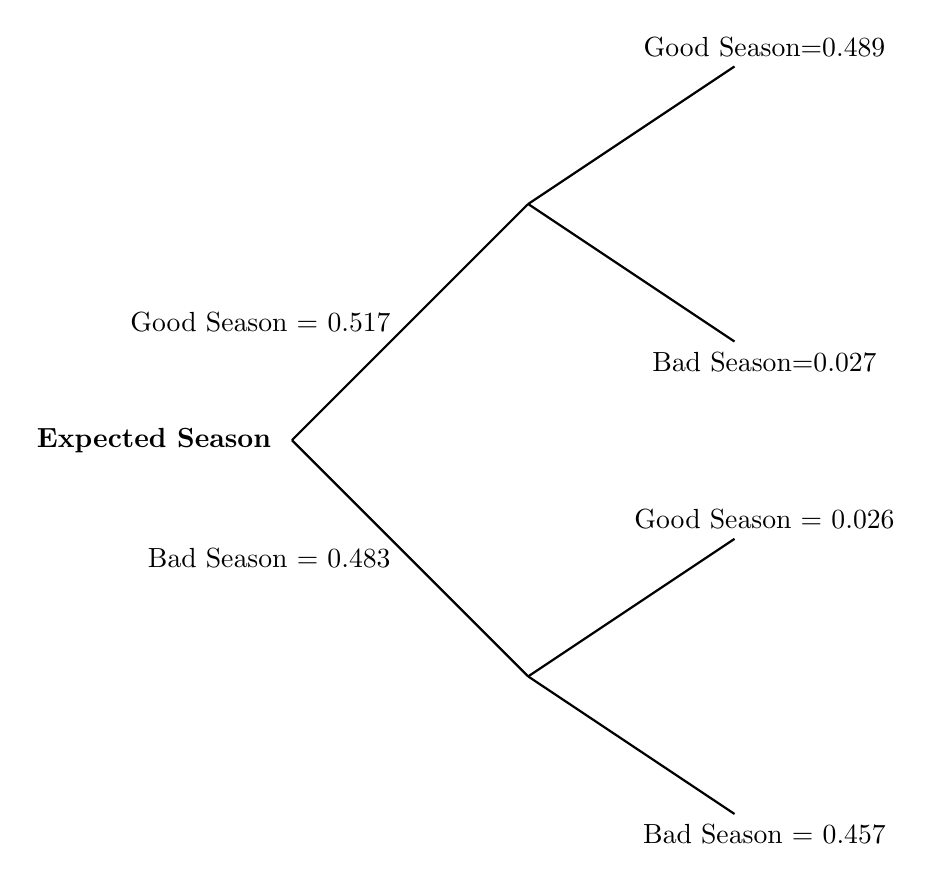
\begin{tikzpicture}[thick,
    level/.style={level distance=3cm},
    level 2/.style={sibling distance=6cm},
    level 3/.style={sibling distance=4cm}
]
\coordinate
child[grow=right, level distance=0pt] {
        child  {
            child {
                node {Bad Season = 0.457}
                edge from parent 
            }
            child {
                node {Good Season = 0.026}
                edge from parent
            }
            edge from parent
            node [left] {Bad Season = 0.483 \ }
        }
        child {
            child {
                node {Bad Season=0.027}
                edge from parent
            }
            child {
                node {Good Season=0.489}
                edge from parent  
            }
            edge from parent 
            node [left] {Good Season = 0.517 \ }
        }
        node [left] {\textbf{Expected Season\ \ }}
    };
\end{tikzpicture}
\end{figure}


\begin{figure}[htpb!]
\caption{Conception and Births: 40-45 Year-olds}
\hspace{8.0cm}\textbf{Realized Season} \vspace{4mm}\\
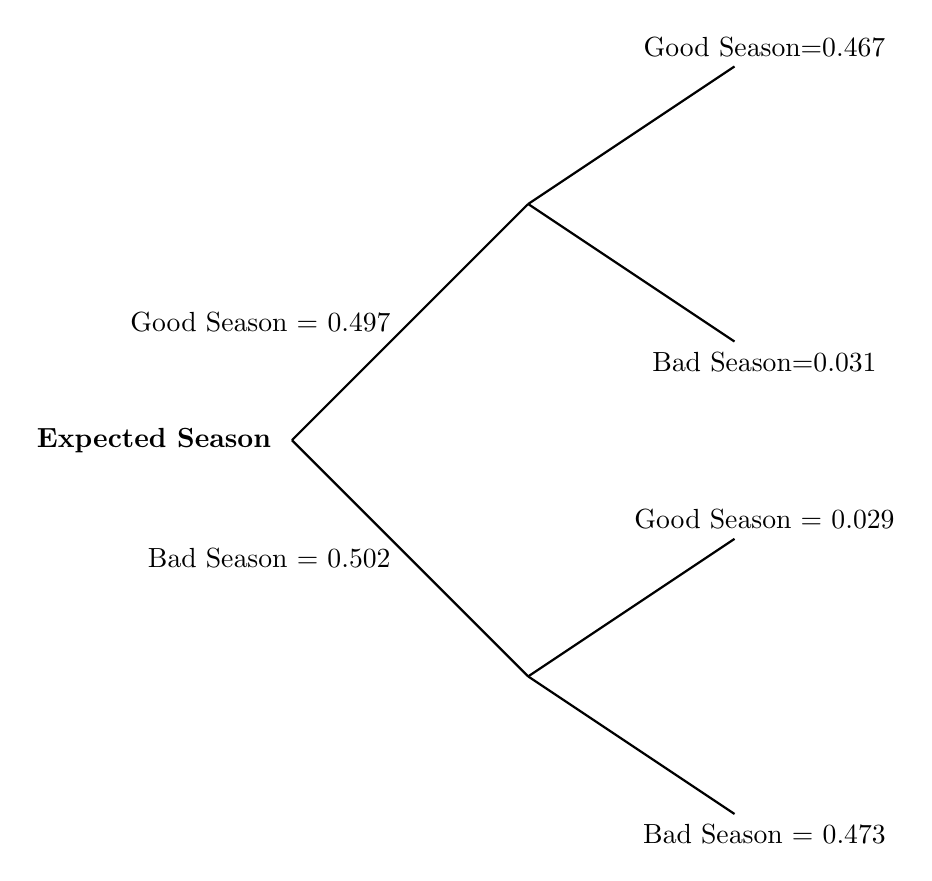
\begin{tikzpicture}[thick,
    level/.style={level distance=3cm},
    level 2/.style={sibling distance=6cm},
    level 3/.style={sibling distance=4cm}
]
\coordinate
child[grow=right, level distance=0pt] {
        child  {
            child {
                node {Bad Season = 0.473}
                edge from parent 
            }
            child {
                node {Good Season = 0.029}
                edge from parent
            }
            edge from parent
            node [left] {Bad Season = 0.502 \ }
        }
        child {
            child {
                node {Bad Season=0.031}
                edge from parent
            }
            child {
                node {Good Season=0.467}
                edge from parent  
            }
            edge from parent 
            node [left] {Good Season = 0.497 \ }
        }
        node [left] {\textbf{Expected Season\ \ }}
    };
\end{tikzpicture}
\end{figure}


\begin{figure}[htpb!]
\begin{center}
  \centering
  \caption{Good Season by State (Young)}
  \includegraphics[scale=0.34]{./../results/nvss/graphs/maps/young.png}
  \label{fig:mapYoung}
\end{center}
\end{figure}

\begin{figure}[htpb!]
\begin{center}
  \centering
  \caption{Good Season by State (Old)}
  \includegraphics[scale=0.34]{./../results/nvss/graphs/maps/old.png}
  \label{fig:mapOld}
\end{center}
\end{figure}

\begin{figure}[htpb!]
\begin{center}
  \centering
  \caption{Temperature and good Quarter: Young (Spain)}
  \includegraphics[scale=0.8]{./../results/spain/graphs/youngTempCold.eps}
  \label{fig:mapYoung}
\end{center}
\end{figure}
\clearpage

\begin{figure}[htpb!]
\begin{center}
  \centering
  \caption{Temperature and good Quarter: Old (Spain)}
  \includegraphics[scale=0.8]{./../results/spain/graphs/oldTempCold.eps}
  \label{fig:mapOld}
\end{center}
\end{figure}

\begin{figure}[htpb!]
\centering
\caption{Child quality: Birthweight (grams)}
\label{QBwt}
\includegraphics[scale=0.8]{../results/nvss/graphs/AllQuality_birthweight_.eps}
\end{figure}
\vspace{1cm}

\begin{figure}[htpb!]
\centering
\caption{Child quality: Birthweight (grams)}
\label{QApgar}
\includegraphics[scale=0.8]{../results/nvss/graphs/Quality_birthweight_.eps}
\end{figure}
\vspace{1cm}





\clearpage
\appendix
\section{Appendix Tables}
\input{./../tables/nvssAppendixTables.tex}

\clearpage
\section{Appendix Figures}
%\begin{figure}[htpb!] 
%\begin{center}
%  \centering  
%  \caption{Education and Conception Month}
%  \includegraphics[scale=0.7]{./../results/nvss/graphs/conceptionMonthDropout.eps}  
%  \label{fig:concepEduc} 
%\end{center}
%\floatfoot{\textsc{Notes to figure \ref{fig:concepEduc}}: Graph plots the proportion
%of conceptions by month for 25-39 year old women by education level.  Refer to figure
%\ref{bqFig:concepMonth} for additional notes.}
%\end{figure} 

\begin{figure}[htpb!]
\centering
\caption{Younger versus older women births (Spain)}
\label{bqFig:YoungvOldSpain}
  \centering
  \includegraphics[scale=0.82]{../results/spain/graphs/youngMonths.eps}
\floatfoot{\textsc{Notes to figure}: Each point and standard error comes from a regression
of birth month $x$ on a binary indicator of being young (25-39).
}
\end{figure}


\begin{figure}[htpb!]
\begin{center}
\caption{Temperature and Good Quarter (Spain)}
\label{fig:tempSpain}
\begin{subfigure}{.5\textwidth}
  \centering
  \includegraphics[scale=0.55]{./../results/spain/graphs/youngTempCold.eps}
  \caption{Young Mothers}
  \label{fig:tempSpainYoung}
\end{subfigure}%
\begin{subfigure}{.5\textwidth}
  \centering
  \includegraphics[scale=0.55]{./../results/spain/graphs/oldTempCold.eps}
  \caption{Old Mothers}
  \label{fig:tempSpainOld}
\end{subfigure}
\end{center}
\floatfoot{\textsc{Notes to figure}: See notes to figure 
\ref{fig:tempUSAYoung}. Monthly temperature data is 
collected from the Spanish State Meteorology Agency (AEMET).}
\end{figure}



\section{Data Appendix}
\label{bqScn:datApp}
\subsection{US Birth Data}
A brief description of US birth certificate data is provided in section
\ref{bqSscn:USAdata} of the paper.  As discussed, the format of US birth
certificates has undergone two important revisions: The first in 1989
and the second in 2003.  The date of adoption of these revisions varies
by state.  By 2013, 41 states or territories had adopted the revised (2003)
format, while the reaminder still follow the 1989 format.\footnote{The full
birth certificate for each revision is reproduced as figures 1 and 2 in
\citet{MenackerMartin2005}.  Over time the adoption of the 2003 certificate
was as follows: 2005: 12 (31\%), 2006: 19 (49\%), 2007: 22 (53\%), 2008: 27
(65\%), 2009: 28 (66\%), 2010: 33 (76\%), 2011: 36 (83\%), 2012: 38 (86\%),
and 2013: 41 (90\%).  In each case the first number refers to the number
of states, while the parenthesis indicates the percent of births in revised
states.}

In all cases where variable coding differs between the revised and unrevised
certificates (principally education for mother and father), we use the revised
2003 coding of the variables.  The reason we do this is because after 2008,
variables which are exclusive to 1989 certificates are no longer reported.
Figure \ref{bqFig:educMissing} illustrates this pattern.  The dotted line
represents the proportion of observations for maternal education which are
reported in the 1989 format, while the bars represent the proportion
\emph{missing} in the 2003 format.  From 2005-2008, all missing 2003 revision
variables are recorded in the 1989 format.  However, from 2009 onwards only
the 2003 revision of education is reported, meaning that those states who
still use the 1989 standard certificate do not have publicly released education
data.  %As expected, these are not missing at random, given that educational
%attainment varies considerably by state (see table \ref{bqTab:missingEduc}).
%In each case when these variables are used, we include full year and state
%fixed effects.




\begin{figure}[htpb!]
\caption{Missing Education Data by Time}
\label{bqFig:educMissing}
\includegraphics[scale=0.74]{../results/nvss/graphs/missingEduc.eps}
\end{figure}
%\input{./../results/nvss/regressions/NVSSMissingScale.tex}


\subsection{Spanish Data}

Birth certificate records from Spain are released by the National Institute of Statistics (INE)
with coverage from 1979 to 2013 inclusive. These consist of the universe of
births registered annually in Spain. Our principal estimation sample consists of
all first born children who survived one day, born to Spanish mothers. We use
births from the period 2007 to 2013, given that prior to 2007, education was not
recorded on birth certificates.  This results in a sample of 1,239,749 live
births, of which 1,238,685 were singletons.

Like birth certificate data in the US, Spanish certificates provide mother
and child characteristics, including education and labour market status of the
mother (and father where present), mother's age at time of birth, marital
status, and child APGAR, gestation, birth weight, prematurity, and so forth
\citep{INE2013}.  The Spanish records include publicly released data on
geographical location of birth, at both the provincial and municipal level
(similar to US states and counties respectively).

Descriptive statistics for Spanish births are provided in table \ref{bqTab:SumStatsSpain}.  In the same
age group, the average age and proportion of young mothers is similar to data
from USA (32 years and 96\% respectively), however a lower proportion report
being married (64\%), or having at least some post secondary education (53\%).
Spanish newborns are slightly lighter on average than their USA-born
counterparts (3,200g), however are also less likely to be born prematurely,
or classified as having low birth weight.

Spanish climate data at the level of the province is calculated from data released by the State Meteorlogical
Agency (AEMET). These data record the temperature at principal state
meteorological stations, from which we calculate monthly average, minima and
maxima.


\section{Tables and Figures Using IPUMS Data (2005-2014)}
\setcounter{figure}{0}  
\renewcommand\thefigure{A.\arabic{figure}}
\setcounter{table}{0}
\renewcommand\thetable{A.\arabic{table}}
\input{./../tables/tablesipums.tex}
\begin{figure}[htpb!]
\centering
\caption{Differences in Prevalence of Good Season Of Birth}
\label{bqFig:YoungvOldIPUMS}
  \centering
  \includegraphics[scale=0.82]{./../results/ipums/graphs/youngQuarter.eps}
\floatfoot{\textsc{Notes to figure}: Each point and standard error comes from a regression
of conception month $x$ on a binary indicator of being young (28-31), versus older (40-45).
}
\end{figure}


\begin{figure}[htpb!] 
\begin{center}
  \centering  
  \caption{Difference in Good Season by Age Group}
  \includegraphics[scale=0.72]{./../results/ipums/graphs/goodSeasonAge.eps}  
  \label{fig:goodByAgeIPUMS} 
\end{center}
\vspace{-5mm}
\floatfoot{\textsc{Notes to figure \ref{fig:goodByAge}}: Coefficients and
standard errors are estimated by regressing ``good season'' on dummies
of maternal age.  Age groups 40-45 are omitted as the base group.  The full
sample consists of mothers aged 20-45.  For the omitted group, proportion 
good season (and standard error) is 0.506(0.008).}
\end{figure} 



\begin{figure}[htpb!]
\begin{center}
\caption{Age and Birth Quarter}
\label{bqFig:birthQuarterIPUMS}
%%\begin{subfigure}{.5\textwidth}
%%  \centering
  \includegraphics[scale=0.72]{./../results/ipums/graphs/birthQuarterAges.eps}
%%  \caption{Proportion of Conceptions in Each Month}
%%  \label{fig:concepAbs}
%%\end{subfigure}%
%%\begin{subfigure}{.5\textwidth}
%%  \centering
%%  \includegraphics[scale=0.55]{./../results/nvss/graphs/conceptionMonthART.eps}
%%  \caption{Proportion of Conceptions (ART Only)}
%%  \label{fig:concepAbsART}
%%\end{subfigure}
\end{center}
\floatfoot{\textsc{Notes to figure \ref{bqFig:birthQuarterIPUMS}}: Birth quarter 
is reported in ACS data. Each line presents the proportion of all births occurring
in each quarter for the relevant age group.}
\end{figure}


\begin{figure}[htpb!]
\begin{center}
\caption{Education and Birth Quarter}
\label{bqFig:concepEducIPUMS}
 \begin{subfigure}{.5\textwidth}
   \centering
   \includegraphics[scale=0.55]{./../results/ipums/graphs/birthQuarterEducYoung.eps}
   \caption{28-31 Year Olds}
   \label{fig:educYoungIPUMS}
 \end{subfigure}%
 \begin{subfigure}{.5\textwidth}
   \centering
   \includegraphics[scale=0.55]{./../results/ipums/graphs/birthQuarterEducOld.eps}
   \caption{40-45 Year Olds}
   \label{fig:educOldIPUMS}
 \end{subfigure}
 \end{center}
 \floatfoot{\textsc{Notes to figure \ref{bqFig:concepEducIPUMS}}: Each line 
presents the proportion of all births conceived in each month for the relevant 
age group and education level. Refer to figure \ref{bqFig:concepMonth} 
for additional notes.}
\end{figure}

 
 \begin{figure}[htpb!]
 \begin{center}
   \centering
   \caption{Good Season by State (Young)}
   \includegraphics[scale=0.7]{./../results/ipums/graphs/youngGoodSeason.eps}
   \label{fig:mapYoungIPUMS}
 \end{center}
 \end{figure}
 
 \begin{figure}[htpb!]
 \begin{center}x
   \centering
   \caption{Good Season by State (Old)}
   \includegraphics[scale=0.7]{./../results/ipums/graphs/oldGoodSeason.eps}
   \label{fig:mapOldIPUMS}
 \end{center}
 \floatfoot{\textsc{Notes to figures \ref{fig:mapYoungIPUMS}-\ref{fig:mapOldIPUMS}}: 
 State data consists of all first births to white non-hispanic women from 2005 
 and 2013.  Figure \ref{fig:mapYoungIPUMS} includes all mothers aged 28-31, while
 figure \ref{fig:mapOldIPUMS} includes mothers aged 40-45.}
 \end{figure}
 
 
 \begin{figure}[htpb!]
 \begin{center}
 \caption{Temperature and Good Quarter}
 \label{fig:tempUSAIPUMS}
 \begin{subfigure}{.5\textwidth}
   \centering
   \includegraphics[scale=0.55]{./../results/ipums/graphs/youngTempCold.eps}
   \caption{Young Mothers (28-31)}
   \label{fig:tempUSAYoungIPUMS}
 \end{subfigure}%
 \begin{subfigure}{.5\textwidth}
   \centering
  \includegraphics[scale=0.55]{./../results/ipums/graphs/oldTempCold.eps}
  \caption{Old Mothers (40-45)}
  \label{fig:tempUSAOldIPUMS}
\end{subfigure}
\end{center}
\floatfoot{\textsc{Notes to figure \ref{fig:tempUSAIPUMS}}: Each point 
represents a state average of the proportion of women giving birth in the 
good birth season between 2005 and 2014.  The dotted line is a fitted 
regression line.  Monthly temperature data is collected from the National 
Centers for Environmental Information.  States with less than 500 births
in ACS over the period of analysis are not displayed.}
\end{figure}

\begin{figure}[htpb!]
  \begin{center}
  \caption{Difference in Births (\% Good Season - \% Bad Season)}
  \label{fig:NVSSbirthsAgesIPUMS}
  \includegraphics[scale=0.8]{./../results/ipums/graphs/birthQdiff_4Ages.eps}
  \end{center}
\end{figure}
%%
%%\begin{figure}[htpb!] 
%%\begin{center}
%%  \centering  
%%  \caption{ART Conceptions by Month}
%%  \includegraphics[scale=0.7]{./../results/nvss/graphs/proportionMonthART.eps}  
%%  \label{fig:ARTMonth} 
%%\end{center}
%%\floatfoot{\textsc{Notes to figure \ref{fig:ARTMonth}}: Proportion of ART births
%%are calculated using data from 2012-2013 for our main sample.  The proportion
%%is calculated as: (ART conceptions)/(Non-ART Conceptions + ART Conceptions).}
%%\end{figure} 
%%
%%\begin{figure}[htpb!]
%%\begin{center}
%%\caption{Difference in Births (\% Good Season - \% Bad Season)}
%%\label{fig:birthDiffART}
%%\begin{subfigure}{.5\textwidth}
%%  \centering
%%  \includegraphics[scale=0.55]{./../results/nvss/graphs/birthQdiff_4AgesART.eps}
%%  \caption{ART Usage}
%%  \label{fig:DiffNoART}
%%\end{subfigure}%
%%\begin{subfigure}{.5\textwidth}
%%  \centering
%%  \includegraphics[scale=0.55]{./../results/nvss/graphs/birthQdiff_4AgesNoART.eps}
%%  \caption{No ART Users}
%%  \label{fig:DiffART}
%%\end{subfigure}
%%\end{center}
%%\end{figure}
%%
\begin{figure}[htpb!]
\begin{center}
\caption{Conceptions by Month (Arizona and Wisconsin)}
\label{fig:conceptionsStatesIPUMS}
\begin{subfigure}{.5\textwidth}
  \centering
  \includegraphics[scale=0.55]{./../results/ipums/graphs/birthQuarterArizonaWisconsin_young.eps}
  \caption{Young Women (28-31)}
  \label{fig:conceptionsStatesYoungIPUMS}
\end{subfigure}%
\begin{subfigure}{.5\textwidth}
  \centering
  \includegraphics[scale=0.55]{./../results/ipums/graphs/birthQuarterArizonaWisconsin_old.eps}
  \caption{Old Women (40-45)}
  \label{fig:conceptionsStatesOldIPUMS}
\end{subfigure}
\end{center}	
\floatfoot{\textsc{Note to figure \ref{fig:conceptionsStatesIPUMS}}: 
Sample consists of all first births from 2005-2013 to white, non-hispanic 25-45 year old 
mothers occurring in the states of Arizona (1,405 births) or Wisconsin (1980 births).}
\end{figure}
%%
%%\begin{figure}[htpb!]
%%  \begin{center}
%%  \caption{Prematurity by Mother's Age}
%%  \label{fig:ARTuse}
%%  \includegraphics[scale=0.8]{./../results/nvss/graphs/prematureAges.eps}
%%  \end{center}
%%\end{figure}
%%



%%NOTE: I TOOK OUT THESE APPENDIX TABLES ON NOV 13 2015.
%%%%\section{Tables Using Conception + 9 Months}
%%%%\setcounter{figure}{0}  
%%%%\renewcommand\thefigure{A.\arabic{figure}}
%%%%\setcounter{table}{0}
%%%%\renewcommand\thetable{A.\arabic{table}}
%%%
%%%%\input{./../tables/tablesexpect.tex}
%%%%\input{./../tables/expectAppendixTables.tex}
%%%
%%%
%%%
%%%%\section{Tables Only For Legally Married Women}
%%%%\renewcommand\thefigure{B.\arabic{figure}}
%%%%\setcounter{figure}{0}  
%%%%\renewcommand\thetable{B.\arabic{table}}
%%%%\setcounter{table}{0}  
%%%%\input{./../tables/tablesmarried.tex}
%%%%\input{./../tables/marriedAppendixTables.tex}


\end{doublespace}
%\end{spacing}
\end{document}







\begin{eqnarray}
\label{struc1}
\max_{\{s,a\}} u(w,b) &\text{s.t.}& w=f(age,educ,\mathbf{X},\varepsilon_w) \\
\label{struc2}
&& b=\mu(age,s,\mathbf{X},\varepsilon_b)                                  \\
\label{struc3}
&& s=\phi(age,educ,\varepsilon_s).
\end{eqnarray}

Here $u(\cdot), f(\cdot), \mu(\cdot)$ and $\phi(\cdot)$ are functions and
$\mathbf{\varepsilon}=(\varepsilon_w,\varepsilon_s,\varepsilon_b)$ are
unobserved shocks.  To close the structural model we must attach functional
form to the four functions, and make distributional assumptions for $\varepsilon$.

Functional form for equations (\ref{struc2}) and (\ref{struc3}) can be quite simple,
as it is precisely what we are estimating in equations (\ref{eqn:season}) and
(\ref{eqn:quality}) respectively.  From our results we know very clearly that:
\[
\frac{\partial b}{\partial s^{good}}>0 \text{\ and \ }
\frac{\partial s^{good}}{\partial age}<0.
\]
It is also generally the case that:
\[
\frac{\partial w}{\partial age}>0.
\]
The wage equation in (\ref{struc1}) could be Mincerian, depending on $age$ and
$age^2$, as well as education, and is calculated at the level of the state,
(perhaps using data from CPS or similar to get wage).  Finally, we define $u(w,b)$
as a Cobb-Douglas
or CES function (or some other logical form), and assume that $\varepsilon$ is
drawn from a trivariate normal.  We can thus write down a log-likelihood function,
and use our birth data to maximise this function, estimating the parameters in
$f(\cdot), \mu(\cdot)$ and $\phi(\cdot)$, which allows us to quantify the
trade-off between ``having a child today'' versus ``having a child tomorrow''
with the relative (market and shadow) prices of labor, as measured by wages, and
child quality, proxied by birthweights.
